\subsection{Excercise DockerEnvironmentSetup}
This exercise sets up the Docker environment.
The goal is to install Docker and run the Hello-World container.

First, Docker is installed on the author's machine.
A quick verification is done to ensure that the installation was successful.
After that, the Hello-World container is run twice explaining the differences between the first and second execution.

\subsubsection*{Installing Docker}
The installation is carried out on the author's machine running Windows 11 with WSL2.
The installation is done by following the official Docker documentation \cite{DO-INST} and the provided guide on the task sheet \cite{CM-G-BSD}.

After successfully installing Docker, the installation is verified by running \texttt{docker \-\-version} and \texttt{docker-compose \-\-version} in the terminal.
The output of the commands is shown in \autoref*{fig:docker_installation_verification}.

\begin{figure}
    \centering
    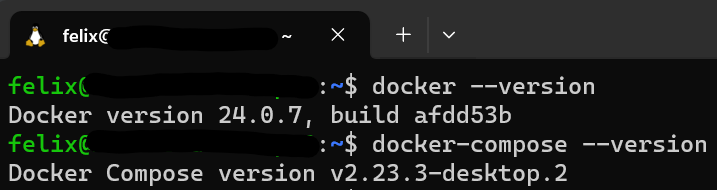
\includegraphics[width=0.8\textwidth]{figures/microservices/dmCar/ms_dmCar_dockerInstallation.png}
    \caption{Docker Installation Verification}
    \label{fig:docker_installation_verification}
\end{figure}
\subsubsection*{Running Hello-World Container}
The next step is to run the Hello-World container.
This is done by running the \texttt{docker run hello-world} command in the terminal.
The command is executed twice showing the differences between both executions.

Execution one is shown in \autoref*{fig:docker_hello_world_first_execution}.
The output shows that the image needed for the container is not available locally at first.
Therefore, the image is pulled automatically from the Docker Hub.
Afterwards, the container is started and the output is shown.

The second execution is shown in \autoref*{fig:docker_hello_world_second_execution}.
Here, the image is already available locally and therefore, no new image needs to be pulled from the Docker Hub.
The container is started instantly and the same output is shown.

\begin{figure}
    \centering
    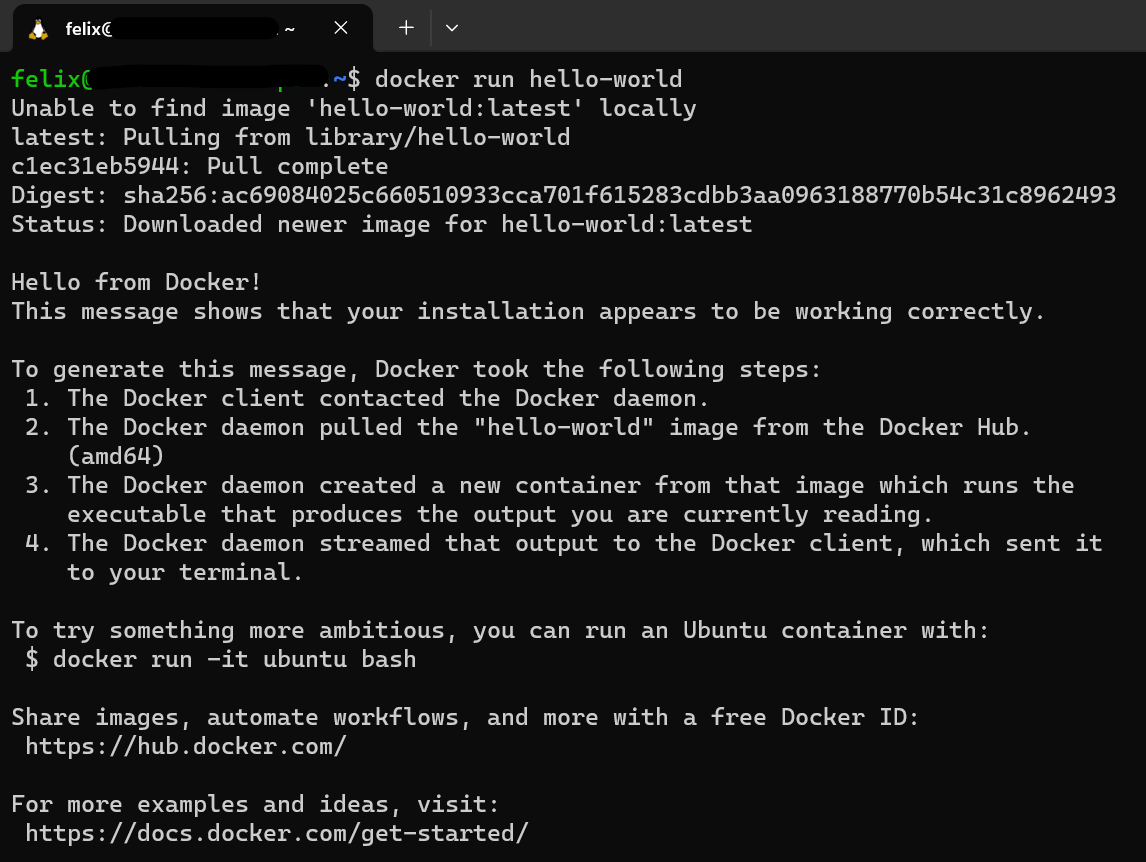
\includegraphics[width=0.6\textwidth]{figures/microservices/dmCar/ms_dmCar_dockerHelloWorldFirstExecution.png}
    \caption{First Execution of Hello-World Container}
    \label{fig:docker_hello_world_first_execution}
\end{figure}

\begin{figure}
    \centering
    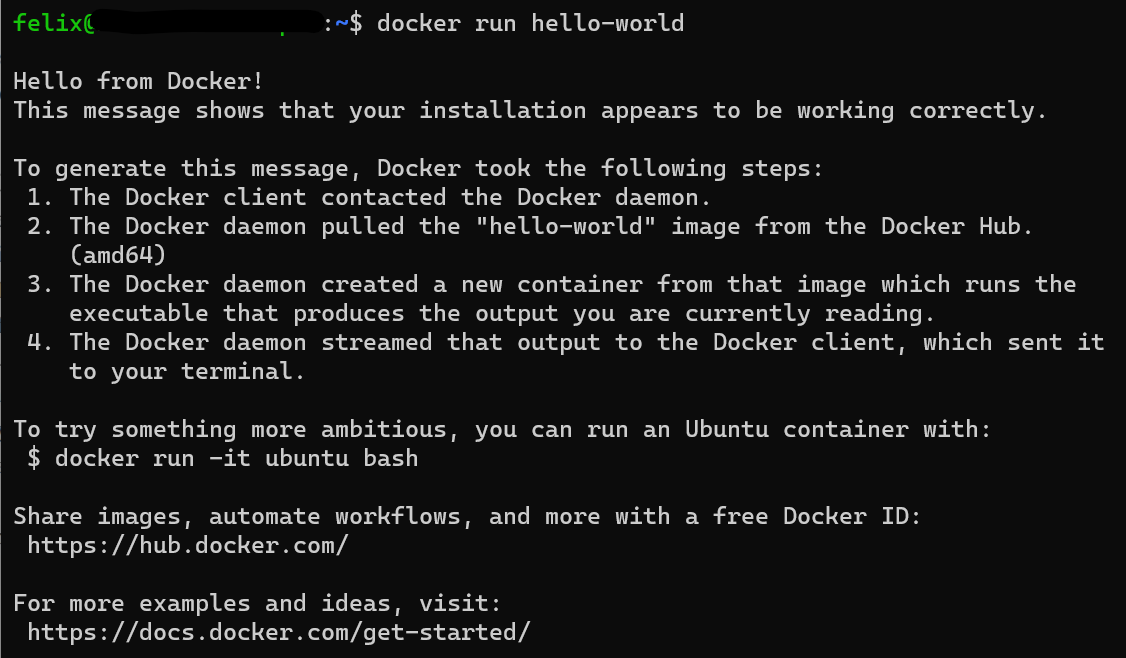
\includegraphics[width=0.6\textwidth]{figures/microservices/dmCar/ms_dmCar_dockerHelloWorldSecondExecution.png}
    \caption{Second Execution of Hello-World Container}
    \label{fig:docker_hello_world_second_execution}
\end{figure}

%==============================================================================

\subsection{Excercise DockerContainerization}
//TODO add introduction
\subsubsection*{Add Dockerfile to DM-Car}
The first step is to add a Dockerfile to the DM-Car project.
This is done by creating a new file called \texttt{Dockerfile} in the root directory of the project.
The content of the file is copied from the Golang project template located at \texttt{1.EngineeringKnowledge/CICD/GolangTemplate}.
After that, the content is pushed to the GitLab repository.

\subsubsection*{Familiarize With Dockerfile Syntax}
The \texttt{dockerfile} is separated into three distinct stages: build, test, and production.
This task analyzes each of them and explains their purpose.
Also, the functionality of the used instructions is explained.

\paragraph*{Build Stage}
The code of the build stage is shown in \autoref*{lst:build_stage_dm_car}.

The build stage builds the go project.
It checks and downloads dependencies, copies and compiles the source code and creates an executable file called \texttt{main}.
This stage, therefore, is the primitive for the following stages.
 
\begin{lstlisting}[
    style=kit-cm,
    caption={Build Stage of the Dockerfile},
    label={lst:build_stage_dm_car},
    float=h
    ]
# ==================
# BUILD STAGE
# ==================
FROM golang:1.21.0-alpine3.18 AS build  # defines the base image that is used for this stage

WORKDIR /app                            # sets the working directory in the container
COPY /src/go.mod /src/go.sum ./         # copies the go.mod and go.sum files from the source directory to the working directory
RUN go mod download                     # runs the go mod download command to download the dependencies
COPY /src/ ./                           # copies the source code from the src directory to the working directory
RUN go build -o main .                  # compiles the source code and creates an executable file called main
\end{lstlisting}

\paragraph*{Test Stage}
The code of the test stage is shown in \autoref*{lst:test_stage_dm_car}.

This stage uses the code from the previous build stage and runs tests on it.
By running it before the production stage integrity of the code is ensured.
If the tests fail, production can be stopped and the code can be fixed ensuring that only working code makes it to the production stage.

\begin{lstlisting}[
    style=kit-cm,
    caption={Test Stage of the Dockerfile},
    label={lst:test_stage_dm_car},
    float=h
    ]
# ==================
# TEST STAGE
# ==================
FROM build AS test      # defines the base image, which is the build stage

RUN go test -v ./...    # runs the 'go test' command to run all tests in the project
\end{lstlisting}

\paragraph*{Production Stage}
The code of the production stage is shown in \autoref*{lst:production_stage_dm_car}.

This is the final production stage.
It uses the \texttt{alpine} image as a base image and copies the essential artifacts from the test stage, which is the main executable, into the production image.
This image only contains the essential artifacts needed to correctly run the application.

\begin{lstlisting}[
    style=kit-cm,
    caption={Production Stage of the Dockerfile},
    label={lst:production_stage_dm_car},
    float=h
    ]
# ==================
# PRODUCTION STAGE
# ==================
FROM alpine:3.18 AS production  # defines the base image, which is the alpine image
                                # the image is then called 'production'

WORKDIR /root/                  # sets the working directory in the container
COPY --from=test /app/main .    # copies the main executable from the test stage to the working directory
EXPOSE 80                       # exposes port 80, which is used by the application
CMD ["./main"]                  # runs the main executable
\end{lstlisting}

\paragraph*{Wrap Up}
The Dockerfile is now complete.
It contains all the necessary stages to build, test, and run the DM-Car application.
The stages are arranged in a way that the build stage is executed first, then the test stage, and finally the production stage.
This ensures that only working code is deployed to the production stage.

Now, the Dockerfile will be used to build a Docker image.

\subsubsection*{Build Docker Image}


\subsubsection*{Optimize Image}


\subsubsection*{Build Optimized Image}


\subsubsection*{Define a File .dockerignore}